\chapter{归约}


\section{归约的概念}

归约实现了问题之间的转化。通常,有些问题是难以直接解决的,

将二部图匹配归约到网络最大流。

将最大权闭包归约到最小割。

子树查询变为区间查询。

GSS2中查询的归约。

区间询问。

\section{SAT问题}

\begin{prob}[合取范式可满足性, CNF-SAT, SAT]
 给定一个合取范式(CNF)表示的逻辑公式$C = C_1 \land C_2 \land \ldots \land C_n$,其中每一个子句(clause) $C_i$都是
 若干变量$x_i$或$\neg x_i$的析取(即或运算连接的)。求每个变量的一个赋值($T$或$F$),使$C$的值为真。例如
 $$(x_1)\land(\neg x_1 \lor x_2)\land(\neg x_2 \lor x_3)$$
 是可满足的,令$x_1=x_2=x_3=T$即可。
\end{prob}

SAT在计算机科学中有着十分重要的地位。对于每一个子句$C_i$中变量的个数不超过2的情况,2-SAT存在十分高效的算法;
但如果仅仅将这个限制放宽为$C_i$中变量个数不超过3,该问题就成为了NP-完全问题,这意味着所有NP问题都可以在多项式时间内归约到
3-SAT,SAT是最早被证明的NP-完全问题。

\begin{prob}[2-SAT]
 在SAT问题中,限制每个子句中包含的变量个数为2个,这样每个子句都是$a\lor b (a \neq b)$的形式,其中$a, b$是变量$x_i$或$x_i$的取反$\neg x_i$。
\end{prob}

解决2-SAT问题的突破口是$(p\to q) = (\neg p \lor q)$。
我们可以将形如$a\lor b$的子句改写成蕴含的形式:$$(a\lor b) = (\neg a \to b) \land (\neg b \to a).$$
这样,2-SAT问题就被我们改写成了若干蕴含式的合取,此时问题的解决也十分明朗:建立有向图$G(V,E)$,其中$V$是由每个变量$x_i$和它的取反$\neg x_i$组成的,
而对于改写后的每一个蕴含式$a\to b$,都在图中添加一条由$a$指向$b$的边。
由于蕴含关系的传递性,若图中如果存在$x_i$到$\neg x_i$的路径,则说明2-SAT中包含矛盾,否则我们就可以依据蕴含关系求出2-SAT的一个解。
更进一步,因为$G$特殊的对称性, $x_i$到$\neg x_i$存在路径总是意味着$\neg x_i$到$x_i$也存在路径,所以2-SAT最终被归约到有向图强连通分量问题的求解。
SAT问题包含了逻辑上的约束关系,因此应用十分广泛,例如下述问题就可以归约到2-SAT:
\begin{prob}
 给定非负整数权无向图$G(V, E, W)$,你需要为每一个结点$v$求一个整数标号$X_v$,使得对于每条边$\{u, v\}\in E$, $X_u \oplus X_v = W_{u,v}$。
 其中$\oplus$为按位异或运算。
\end{prob}

除了在计算理论中的价值外,SAT问题还有其实际应用。因为其NP-完全的特性,很多问题都可以十分容易地归约到SAT问题,
SAT也因此成为解决许多难问题的标准途径。
人们对SAT问题求解的需求增长,也刺激了对SAT问题求解的研究。尽管SAT问题在理论上是十分困难的,但很多算法确实能非常高效地解决各种实际问题,
能够求解现实问题中数万个变量、数百万个子句的SAT问题,我们能从互联网上获取各种各样的SAT solver。

\begin{prob}[覆盖问题, Exact Cover, EC]
 给定一个$n\times m$的01矩阵$A$,求一个行的集合$C\subseteq[n]$,满足对于任意的$j$, 
 $\sum_{i\in C} A_{i,j} = 1$。也就是说,我们要从$A$中取出若干行得到一个子矩阵,满足该子矩阵中每列恰好只有一个$1$。
 例如,若
 $$A = 
 \begin{pmatrix}
  0 & 0 & 0 & 1 & 0 & 1\\
  1 & 1 & 1 & 1 & 0 & 0\\
  1 & 0 & 1 & 0 & 1 & 0\\
  0 & 1 & 0 & 0 & 0 & 0\\
 \end{pmatrix},
 $$
 则$C=\{1, 3, 4\}$是一个合法的覆盖,而$\{1, 2, 4\}$则不是。
\end{prob}

% SPOJ 217
% 你在玩一个塔防小游戏,游戏在一张矩形地图上进行,地图上有4种格子,分别是防御塔、敌人、障碍和空地。你只能在游戏开始前调整防御塔的状态,虽然游戏开始以后敌人是不会动的,但你的目标是消灭所有的敌人,并保证防御塔之间不会误伤。

Exact Cover是一个NP-完全问题,使用Dancing Links数据结构的搜索配合一些启发策略是解决Exact Cover问题的通常手段。
为了充分利用SAT solver,我们现在将Exact Cover归约到SAT:我们为矩阵的每一行设置一个变量$x_i$,当$x_i=T$时,我们希望$i\in C$,相反当$x_i=F$时,$i\notin C$。
首先,我们希望矩阵中的每一列都被覆盖,因此对于每一列$j$,令$T_j = \{ i~|~ A_{i,j} = 1\}$, 则子句
$$\bigvee_{i \in T_j} x_i$$
代表了``第$j$列至少包含一个1''。
其次,我们希望每一列至多只有一个1。因此我们必须禁止某些行被同时选中,即对于每一对$(p,q)$,若第$p$行和第$q$行在同一列上有公共的1,我们需要满足
$$\neg (x_p \land x_q) = (\neg x_p \lor x_q).$$

将$n\times m$规模的Exact Cover归约到SAT问题后约有$O(m)$个$O(n)$大小的clause,以及$O(n^2)$个$O(1)$大小的clause,问题的整体规模并没有数量级上的提升,
这个归约可以用来解决很多问题,例如数独的求解。

\begin{prob}[新数独问题]
 你需要在一个$16\times16$的方阵中填入A-P这16个字母,并且满足每行、每列以及16个粗线标出的$4\times4$方格中,A-P中的每个字母恰好出现一次。
 固定方阵中的一些字母,求一组可行的解。问题的例子如图 \ref{fig:SUDOKU} 所示。
 \begin{figure}
  \center
  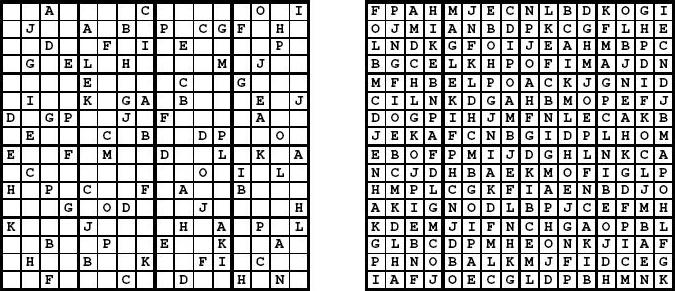
\includegraphics[width=400pt]{sudoku.png}
  \caption{新数独问题}
  \label{fig:SUDOKU}
 \end{figure}
\end{prob}

在数独的例子中,我们生成的SAT问题有$4096$个变量,$10^5$数量级的约束条件,但一个好的SAT solver仍然能够在数秒以内给出正确的解答。